%TODO Final reread for english
%TODO Final formatting
%TODO We need a hypothesis or else we lose points

\documentclass[12pt]{article}
\usepackage{mathtools, amsmath, amsfonts, amssymb}
\usepackage{hyperref, graphicx, wrapfig, geometry}
\usepackage[makeroom]{cancel}
\usepackage{placeins}
\usepackage{float}


\newgeometry{margin=2cm}

\title{Microprocessor Systems - Lab 2 Report}
\author{Auguste Lalande, Felix Dube, Juan Morency Trudel}
\date{\today}

\begin{document}
\maketitle
\clearpage

\tableofcontents
\clearpage

\section{Abstract}
Today's microprocessors inevitably need temperature monitoring to avoid overheating. To this end, the goal of this experiment was to acquire, analyse, and output the built in temperature sensor data on the STM32F4DISCOVERY board's STM32F4407VGT6 processor. A key point of the data processing was noise reduction which was achieved using a 1-D Kalman filter. The data was then converted to temperature values and displayed on four 7-segment displays as well as a small LCD. Lastly, an overheating alarm was implemented.

\section{Problem Statement}
\subsection{ADC configuration} Since the temperature sensor measurements are mapped into a voltage range and not directly into digital data, an analog to digital converter (ADC) on the microprocessor has to be correctly used. In this kind of digitization, sampling frequency must be high enough to have enough time resolution but as low as possible for energy and processor time considerations.
\subsection{Filtering}
Some kind of filtering has to be applied to the input data in order to overcome the noise induced by the sensor and the ADC inaccuracies. Filtering parameters for the chosen implementation have to be tuned to the context of temperature measurement for overheating detection.
\subsection{Data conversion}
Data from the ADC is read by the microcontroller as a 12-bit unsigned integer which must be mapped to a temperature value for it to have a significance to the human observer.
\subsection{Display}
Visual feedback is required in this experiment. The type of display and configuration parameters such as refresh rate have to be chosen to best represent the incoming data.
\subsection{Overheating alarm}
Another visual feedback is required to inform the user of overheating. The right threshold to activate this alarm has to be chosen.

\section{Theory and Hypothesis}
\subsection{Kalman filter}
\label{kalman_filter}
Signals like the temperature recorded in this experiment can be affected by noise of different nature: thermal noise, interference, quantum noise, shot noise, etc \cite{kuo1995active}. Most of these noises are random in nature thus the need to use some kind of filter instead of simply adjusting the ADC conversion formula. For varying processes like the temperature, an adaptive approach is usually preferred \cite{kuo1995active}. Of the many algorithms that exist for noise filtering in a signal, the Kalman filter algorithm \cite{kalman1960new} has been praised for its fast and elegant recursive design. Because of the Gaussian nature of most of the noise present in this experiment \cite{kish2000noise}, the Kalman filter is a natural choice. 

A Kalman filter algorithm usually has state variables to model the noise and adjust the value of the filtered data. Each time a new input is filtered, these state variables are recalculated to model the changing environment. Parameters that are used in this experiment will be: $k$ the  adaptive  tuning  factor, $p$ the covariance on the estimation error, $q$ the noise parameter in the  input  measurements,  and $r$ the noise parameter in the  state  estimation. While $k$ and $p$ are updated on every measurement, $q$ and $r$ are not and are important to specify in order to have a enough smoothing while having a reasonable convergence time \cite{kalman1960new}. The choice of these parameters is explained in section \ref{kalman_filter_params}.

\subsection{Systick and Timing}
Systick is a process that counts the period of the processor clock. It starts a counter at a specified value and decrements it each clock cycle. When the counter reaches to 0, the Systick handler is called \cite{STMCubeDatasheet}. This will be used to set up various timing requirements of the project.

\subsection{Hypothesis}
Although the microcontroller temperature sensor is of low quality, the time proven reliability of the kalman filter suggests that displaying temperature data with reasonable accuracy will be possible. 

\section{Implementation}

The implementation of our system is briefly described in the next sections. For a more complete explanation of the software, please refer to the code. 

\subsection{Analog to Digital Converter}
A single ADC channel was configured with key parameters shown in table \ref{ADC_config}. First, channel 16 was chosen since the internal temperature sensor is hard wired to it. Next, because temperature is varying slowly it was decided that a 100 Hz sampling frequency was enough. For this purpose, a slower clock ($168/4 = 42$ MHz) and the slowest sampling time was chosen. The resolution was set at 12 bits to have the maximum precision in the reading. Finally, the 12 bit data was aligned to the right in a 32 bit word to facilitate data processing.
\begin{table}[H]
\centering
\caption{Key Parameters of the ADC Initialization}
\label{ADC_config}
\begin{tabular}{|l|l|}
\hline
\multicolumn{1}{|c|}{\textbf{Parameter}} & \multicolumn{1}{c|}{\textbf{Value}} \\ \hline
Channel                                  & ADC\_CHANNEL\_16                    \\ \hline
SamplingTime                             & ADC\_SAMPLETIME\_480CYCLES          \\ \hline
ClockPrescaler                           & ADC\_CLOCK\_SYNC\_PCLK\_DIV4        \\ \hline
Resolution                               & ADC\_RESOLUTION\_12B                \\ \hline
DataAlign                                & ADC\_DATAALIGN\_RIGHT               \\ \hline
\end{tabular}
\end{table}

\subsection{General Purpose Input Output}
\FloatBarrier
GPIO pins were used to interface with the 7-segment displays, the LCD and the alarm LEDs. The pins on ports B, D, and E were used for their availability. For maximum speed, the pins were set to push-pull mode and the speed parameter was set to medium due to the maximum speed of the GPIO pins on the STM32F4407VGT6 being $48 MHz$ \cite{STM32F407xx}.

\subsection{Filtering}
Smoothing of the temperature readings was implemented using a one dimensional kalman filter with the parameters mentioned in section \ref{kalman_filter}. The parameter values were chosen through trial and error.

\subsection{Systick and Timing}
For the timing flexibility required in the software, the Systick period was set at $1\mu s$. From there, task dedicated counters were incremented each time the Systick interrupt was called. The $1\mu s$ time was especially important to configure the LCD effectively. One counter was used for the ADC sampling period, and 5 for the displays for a total of 6. The various utilities of the timers for the displays are explained in sections \ref{7seg_dis} and \ref{LCD_dis}.
\subsection{7-Segments Displays}
\label{7seg_dis}

To control the 7-segment displays, 8 pins on port B of the microcontroller were dedicated to selecting which segments and/or decimal point should be turned on or off, by setting the pins to high or low respectively. Additionally, 3 pins were used to select which of the available 7-segment displays should be displaying the data indicated on the first 8 pins. This was done by connecting each pin to a PNP transistor which would only let current flow through the selected 7-segments. Our code would then cycle through each display each time changing the digit to being shown. When done fast enough, it would look to the eye as if all displays were on simultaneously.

To control the display time of the 7 segment display, 2 counters were used. A first counter called \textit{display7segTimer} was used to set the frequency at which the display function is called (a kind of refresh rate) and a second counter was used to limit the speed at which the incoming value to be displayed is changed. These values were adjusted to have minimum dimming of the display and to avoid flickering through trial and error.

\subsection{LCD Display}
\label{LCD_dis}
An alternative way of presenting the temperature is to use an LCD display. The display used for this experiment is an LCD based on  the  Hitachi  HD44780  controller  chipset made by Sparkfun with part number GDM1602k. The processor communicates with the display using 2 control bits and an 8-bit data bus. On the display, each character position is an address in memory (memory of the display itself). In order to write something on the display, a character needs to be saved at the appropriate memory address. The basic built in functions of the HD44780 controller interfaced with the GPIO E port were used to display characters. Simple type casting was used to convert the float temperature to be display into a char array. The display gets updated at the same reduced frequency (2 Hz) of the 7 segment display to improve readability. 

\subsection{Overheating Alarm}
A trivial overheating alarm was implemented by verifying at each temperature measurement if the value is above a threshold. To avoid false positive, the filtered data is used in the overheating verification. Additionally, five consecutive values above threshold have to be recorded for the alarm to turn on. The alarm threshold was set to $42.5^\circ$ Celsius for testing purposes but would be set a little lower than the junction temperature for the actual system in the actual system. In this implementation, the alarm routine doesn't actually try to cool down the processor but simply makes some LEDs on the board blink to warn the user.

\subsection{Code structure}
 Figure \ref{fig:statediagram} present the state diagram of our implementation. Each timer variables are incremented in the systick handle.

\begin{figure}[!htb]
\centering
\includegraphics[scale=0.6]{images/statediagram.png}
\caption{State Diagram of the Temperature Monitoring Software}
\label{fig:statediagram}
\end{figure}


\section{Testing and Observations}

\subsection{Kalman Filter Parameters}\label{kalman_filter_params}
As mentioned in section \ref{kalman_filter}, the parameters for the kalman filter had to be optimized for the application of temperature monitoring. Adjustments were done by trial and error for parameters $q$ and $r$. Figure \ref{fig:kalmanfilter} shows the input and output data of the filter with and without tuned parameters. The time of convergence that can be observed in this figure is roughly 30 measurements which corresponds to about 300 ms. This was judged to be sufficient because temperature varies relatively slowly in the processor (it will not jump by 50 degrees in less than a second). The $k$ and $p $parameters were set to the values they were expected to converge to after running the filter for a long period. Nevertheless, the initial value of $k$ and $p$ proved to have close to no impact on the resulting filter characterization.
\begin{figure}[!htb]
\centering
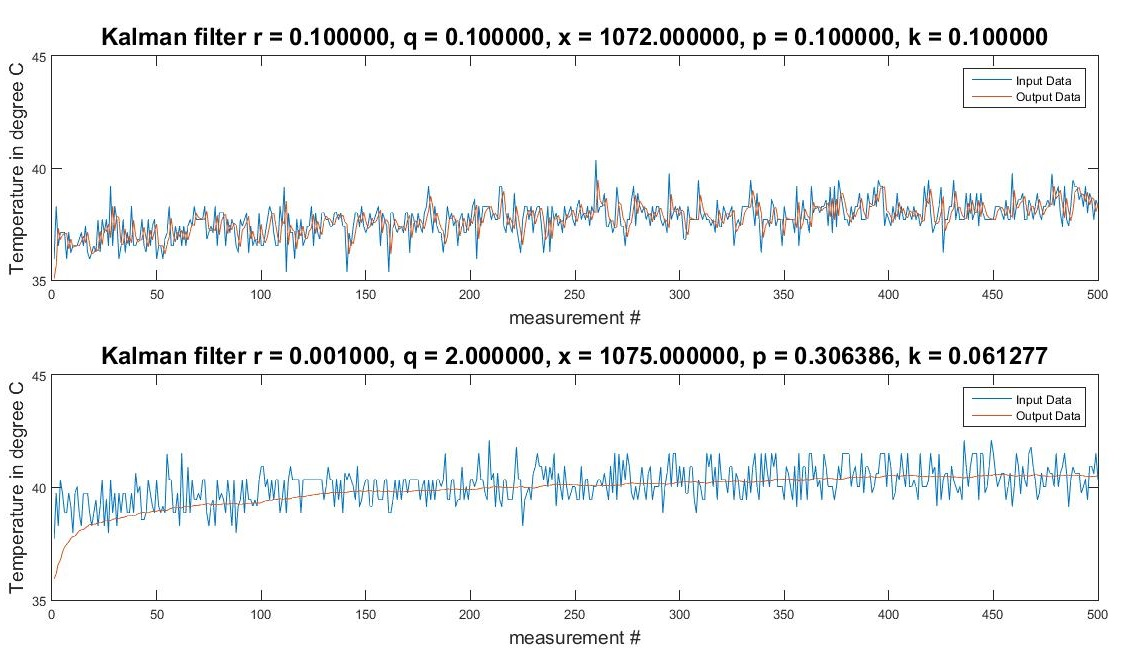
\includegraphics[scale=0.50]{images/kalmanfilter.jpg}
\caption{Filtered Data Compared to Raw Data Before and After Optimising the Kalman Filter Parameters}
\label{fig:kalmanfilter}
\end{figure}

\subsection{Display}
In order to achieve an acceptable display, timing parameters for the 7-segment display were tested by trial and error. In order for the 7-segment display to operate properly, 2 parameters had to be adjusted: the time before the next digit gets shown and the number of times a single digit gets refreshed per second. At first, our algorithm just cycled through the digits at maximum speed, but this proved to be too fast for the human eye (the LEDs were not staying on long enough). To make up for this, the counter \textit{timeDisplay1DigitTimer} was used to wait $2ms$ before changing the digit to display. This was the maximum value that did not cause noticeable flickering. The second parameter, the refresh rate of a single digit was tuned at the minimum Systick time of $1/mu s$. Due to the nature of our implementation which turns on and then directly off the LEDs in one function call, the function has to be called as much as possible to avoid dimming on the LED. Needless to mention that this limitation can be overcome by improving our display algorithm.

\section{Conclusion}
The objective of this experiment was to set up the required drivers in order to measure and display the temperature in the processor and implement an overheating alarm. The results suggests that filtering the data was indeed important to avoid falsely triggering the alarm and accurately monitor temperature. Additionally, controlling the timing of the system proved to be essential especially for the correct operation of the ADC and the display. Overall this experiment demonstrated the importance of temperature monitoring in electronic applications.

\newpage
\section{Bibliography}
\bibliographystyle{unsrt}
\bibliography{LabReport2} 
\end{document}
